%\documentclass[tikz, border=5pt]{standalone}
\begin{document}
	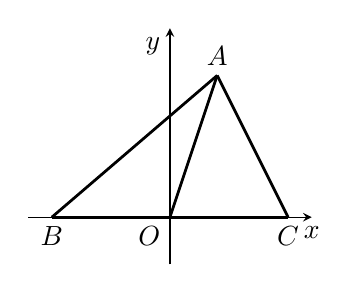
\begin{tikzpicture}[>=stealth, scale=0.6] % 箭头样式为stealth,
		
		% 绘制坐标轴
		\draw[->] (-3,0) -- (3,0) node[below] {$x$};      % x轴(带箭头和标签)
		\draw[->] (0,-1) -- (0,4) node[below left] {$y$}; % y轴(带箭头和标签)
		\node at (0,0) [below left] {$O$};                % 原点O的标签
		
		% 定义各关键点坐标
		\coordinate (A) at (1,3);    % 点A
		\coordinate (B) at (-2.5,0); % 点B
		\coordinate (C) at (2.5,0);  % 点C
		\coordinate (O) at (0,0);   % 原点 O
		
		% 绘制连接点的直线
		\draw[line width=1pt] (A) -- (B);
		\draw[line width=1pt] (A) -- (C);
		\draw[line width=1pt] (A) -- (O);
		\draw[line width=1pt] (B) -- (C);
		
		% 标记各点的标签
		\node at (B) [below] {$B$};
		\node at (A) [above] {$A$};
		\node at (C) [below] {$C$};
		
	\end{tikzpicture}
\end{document}
